\documentclass[aspectratio=169,11pt]{beamer}

\usetheme{Madrid}
\usecolortheme{seahorse}
\usefonttheme{professionalfonts}

\usepackage[T1]{fontenc}
\usepackage{lmodern}
\usepackage{amsmath,amssymb}
\usepackage{booktabs}
\usepackage{graphicx}
\usepackage{xcolor}
\usepackage{hyperref}
\usepackage{tikz}
\usetikzlibrary{shapes.geometric,arrows.meta,positioning,fit,backgrounds}

% The deck is compiled from docs/, while its media bundle lives in ppt_assets/.
\graphicspath{{../ppt_assets/}}

\definecolor{hgpurple}{RGB}{106,61,154}
\definecolor{softblue}{RGB}{63,107,160}
\definecolor{softgreen}{RGB}{44,160,137}
\definecolor{softorange}{RGB}{220,139,42}

\setbeamertemplate{navigation symbols}{}
\setbeamertemplate{caption}[numbered]
\setbeamercolor{title}{fg=hgpurple}
\setbeamercolor{frametitle}{fg=hgpurple}
\setbeamercolor{structure}{fg=hgpurple}

\newcommand{\safeimage}[2][]{\includegraphics[#1]{../ppt_assets/#2}}
\newcommand{\abimage}[2][]{\includegraphics[#1]{"../ablation styudy/figures/#2"}}

% 2x2 grid of graphs on one slide, with a compact caption line
\newcommand{\quadfigs}[6]{
  \begin{frame}{#1}
    \centering
    \begin{columns}[T,totalwidth=\linewidth]
      \begin{column}{0.49\linewidth}
        \centering
        \safeimage[width=\linewidth,height=0.31\textheight,keepaspectratio]{#2}\\[2mm]
        \safeimage[width=\linewidth,height=0.31\textheight,keepaspectratio]{#4}
      \end{column}
      \begin{column}{0.49\linewidth}
        \centering
        \safeimage[width=\linewidth,height=0.31\textheight,keepaspectratio]{#3}\\[2mm]
        \safeimage[width=\linewidth,height=0.31\textheight,keepaspectratio]{#5}
      \end{column}
    \end{columns}
    \vspace{1.5mm}
    {\tiny #6}
  \end{frame}
}

% 3-across row of graphs on one slide, with room for bullets below
\newcommand{\trifigsnote}[5]{
  \begin{frame}{#1}
    \centering
    \begin{columns}[T,totalwidth=\linewidth]
      \begin{column}{0.32\linewidth}
        \centering
        \safeimage[width=\linewidth,height=0.4\textheight,keepaspectratio]{#2}
      \end{column}
      \begin{column}{0.32\linewidth}
        \centering
        \safeimage[width=\linewidth,height=0.4\textheight,keepaspectratio]{#3}
      \end{column}
      \begin{column}{0.32\linewidth}
        \centering
        \safeimage[width=\linewidth,height=0.4\textheight,keepaspectratio]{#4}
      \end{column}
    \end{columns}
    \vspace{2mm}
    {\scriptsize #5}
  \end{frame}
}

\tikzstyle{stage}=[rectangle, rounded corners, draw=hgpurple, thick,
  fill=hgpurple!8, text width=3.05cm, align=center, minimum height=1.05cm,
  font=\scriptsize]
\tikzstyle{force}=[rectangle, rounded corners, draw=softorange, thick,
  fill=softorange!12, text width=2.5cm, align=center, minimum height=0.9cm,
  font=\tiny]
\tikzstyle{arrow}=[-{Latex[length=2mm]}, thick, softblue]

\title[Hamiltonian-Geometric Optimization]{Hamiltonian-Geometric Optimization Framework for Machine Learning}
\subtitle{A Concise Walkthrough: Framework, Validation, Evidence}
\author[Chakraborty et al.]{Sparsho Chakraborty \and Mohammad Alamgir \and Adreet Sarkar \and Nishant M}
\institute{Capacitor Fringes Project}
\date{\today}

\begin{document}

% ---------- 1. Title ----------
\begin{frame}
  \titlepage
\end{frame}

% ---------- 2. Motivation / Core Question ----------
\begin{frame}{Core Question}
  \begin{block}{Goal}
    Can a single \textbf{Hamiltonian-geometric} update rule act as a useful optimizer family
    across classical ML, LLM-style training, PINNs, and quantum-control objectives?
  \end{block}
  \begin{itemize}
    \item Treat parameters $\theta$ as generalized coordinates, the loss $L(\theta)$ as potential
      energy, and optimizer state as momentum $p$ evolving on a \textbf{metric manifold} $g(\theta)$.
    \item One family should recover SGD, momentum, Adam, and natural gradient as special cases.
    \item Claim is deliberately \emph{bounded}: not uniformly superior, strongest when full-metric
      curvature is exploitable.
  \end{itemize}
\end{frame}

% ---------- 3. Mathematical framework as a flowchart ----------
\begin{frame}{Methodology --- Mathematical Framework at a Glance}
  \centering
  \resizebox{\linewidth}{0.68\textheight}{
  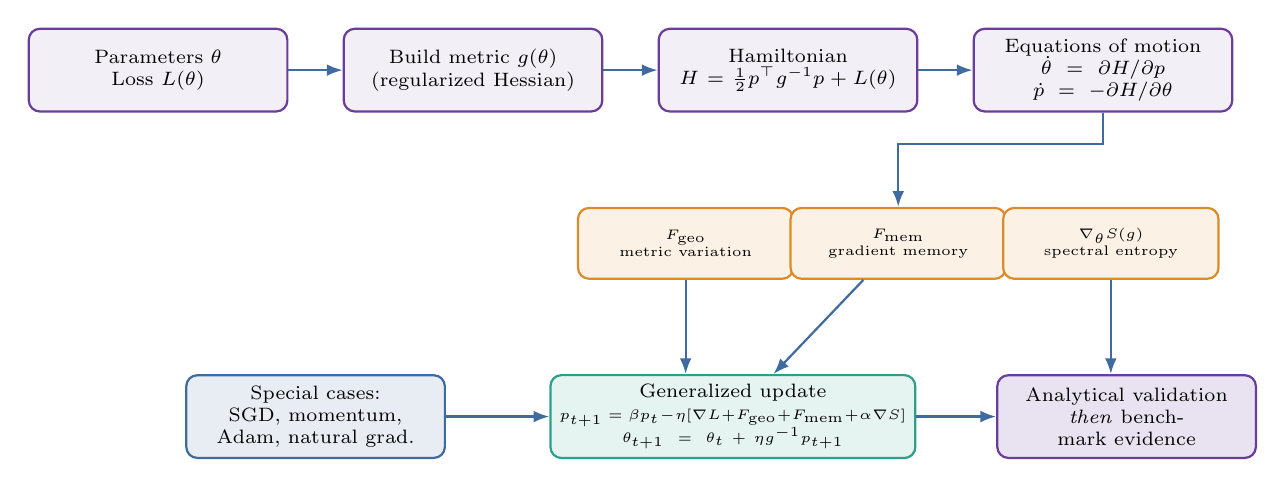
\begin{tikzpicture}

    % Row 1: deterministic setup, left to right
    \node[stage] (in) at (0,0) {Parameters $\theta$\\ Loss $L(\theta)$};
    \node[stage] (metric) at (4.0,0) {Build metric $g(\theta)$\\ (regularized Hessian)};
    \node[stage] (ham) at (8.0,0) {Hamiltonian\\ $H=\tfrac12 p^{\top}g^{-1}p+L(\theta)$};
    \node[stage] (eom) at (12.0,0) {Equations of motion\\ $\dot\theta=\partial H/\partial p$\\ $\dot p=-\partial H/\partial\theta$};

    % Row 2: three correction forces, centered below row 1
    \node[force] (fgeo) at (6.7,-2.2) {$F_{\mathrm{geo}}$\\ metric variation};
    \node[force] (fmem) at (9.4,-2.2) {$F_{\mathrm{mem}}$\\ gradient memory};
    \node[force] (fent) at (12.1,-2.2) {$\nabla_\theta S(g)$\\ spectral entropy};

    % Row 3: merged update, special cases, and validation
    \node[stage, fill=softblue!12, draw=softblue] (cases) at (2.0,-4.4)
      {Special cases:\\ SGD, momentum,\\ Adam, natural grad.};
    \node[stage, fill=softgreen!12, draw=softgreen, text width=4.4cm] (update) at (7.3,-4.4)
      {Generalized update\\[2pt] \tiny $p_{t+1}=\beta p_t-\eta[\nabla L+F_{\mathrm{geo}}+F_{\mathrm{mem}}+\alpha\nabla S]$\\
       \tiny $\theta_{t+1}=\theta_t+\eta g^{-1}p_{t+1}$};
    \node[stage, fill=hgpurple!15] (valid) at (12.3,-4.4)
      {Analytical validation\\ \emph{then} benchmark evidence};

    \draw[arrow] (in) -- (metric);
    \draw[arrow] (metric) -- (ham);
    \draw[arrow] (ham) -- (eom);
    \draw[arrow] (eom.south) -- ++(0,-4mm) -| (fmem.north);
    \draw[arrow] (fgeo) -- (update.north -| fgeo);
    \draw[arrow] (fmem) -- (update);
    \draw[arrow] (fent) -- (update.north -| fent);
    \draw[arrow] (cases) -- (update);
    \draw[arrow] (update) -- (valid);

  \end{tikzpicture}}

  {\tiny Deterministic stages left to right; forces merge into one update rule; output feeds
  validation before benchmarking.}
\end{frame}

% ---------- 4. Hamiltonian formulation ----------
\begin{frame}{Hamiltonian Formulation}
  \small
  \begin{align*}
    H(\theta,p) &= \frac{1}{2}p_i g^{ij}(\theta)p_j + L(\theta),\\
    \dot{\theta}^{i} = \frac{\partial H}{\partial p_i} &= g^{ij}(\theta)p_j, \qquad
    \dot{p}_i = -\frac{\partial H}{\partial \theta^i}
      = -\partial_i L - \frac{1}{2}p_j p_k\,\partial_i g^{jk}(\theta).
  \end{align*}
  \begin{itemize}
    \item Second term in $\dot p_i$ is the \textbf{geometric force} from a coordinate-dependent metric.
    \item Dissipation is added so dynamics \emph{optimize} rather than conserve energy.
    \item Same structure carries the memory and spectral-entropy correction terms.
  \end{itemize}
\end{frame}

% ---------- 5. Update rule / special cases (condensed) ----------
\begin{frame}{One Update Rule, Many Optimizers}
  \scriptsize
  \begin{tabular}{@{}p{0.24\linewidth}p{0.68\linewidth}@{}}
    \toprule
    Optimizer & Hamiltonian-geometric specialization \\
    \midrule
    SGD / heavy-ball & Flat metric, $F_{\mathrm{geo}}=0$, instant or finite momentum relax \\
    Adam / RMSProp & Diagonal adaptive metric; ignores $F_{\mathrm{geo}}$ from metric variation \\
    Natural gradient & Full information metric, usually no momentum or memory force \\
    Hamiltonian-geometric & Full metric \emph{with} momentum, memory, spectral entropy, curvature \\
    \bottomrule
  \end{tabular}
  \vspace{1em}
  \begin{itemize}
    \item Modern optimizers (Shampoo, K-FAC, Muon, AdaFactor, LARS/LAMB) sit at intermediate
      points on the same metric-structure hierarchy --- from full $n\times n$ down to a single
      global scalar.
  \end{itemize}
\end{frame}

% ---------- 6. Analytical validation ----------
\begin{frame}{Analytical Validation (Equation-Level, All PASS)}
  \footnotesize
  \textbf{What \& reference:} each row checks one equation from Sparsho Chakraborty's
  \emph{literature-review PDF} --- the design reference for this optimizer's architecture ---
  against a finite-difference computation on a fixed, seeded, genuinely curved-metric toy problem.
  \vspace{0.4em}

  \scriptsize
  \begin{tabular}{@{}p{0.4\linewidth}p{0.1\linewidth}rrl@{}}
    \toprule
    Check & Kind & Max error & Tol. & Result \\
    \midrule
    Legendre transform & literal & $2.96\times10^{-11}$ & $10^{-6}$ & PASS \\
    Geometric force & literal & $4.60\times10^{-11}$ & $10^{-5}$ & PASS \\
    Flat-metric reduction & literal & $0.000$ & $10^{-9}$ & PASS \\
    Memory recursion & literal & $8.88\times10^{-16}$ & $10^{-9}$ & PASS \\
    Hessian regularization & counterex. & $0.000$ & $10^{-9}$ & PASS \\
    Rayleigh dissipation (curved metric) & completed & $1.64\times10^{-9}$ & $10^{-6}$ & PASS \\
    Spectral entropy gradient & completed & $1.14\times10^{-10}$ & $10^{-5}$ & PASS \\
    \bottomrule
  \end{tabular}
  \vspace{0.6em}
  \begin{itemize}
    \item \textbf{literal} = tests a PDF equation exactly as printed; \textbf{completed} = tests our
      documented completion of a formula the PDF states but never fully derives; \textbf{counterex.}
      = shows the PDF's literal condition fails, then confirms the shipped code fix succeeds.
  \end{itemize}
\end{frame}

% ---------- 7. Benchmark evidence (4 graphs, one slide) ----------
\quadfigs
  {Benchmark Evidence Snapshot}
  {test_result_media/mnist_optimizer_benchmark/mnist_test_accuracy.png}
  {test_result_media/algoperf_style_hg_nonzero_150epochs/algoperf_style_validation_loss.png}
  {test_result_media/deepobs_style_benchmark/deepobs_style_accuracy.png}
  {test_result_media/industry_llm_benchmark_wikitext2_200steps/industry_llm_validation_loss.png}

% ---------- 8. Classical, PINN & LLM benchmark table ----------
\begin{frame}{Benchmark Results --- Classical, PINN \& LLM}
  \scriptsize
  \begin{tabular}{@{}p{0.24\linewidth}p{0.26\linewidth}p{0.24\linewidth}p{0.18\linewidth}@{}}
    \toprule
    Workload & Hamiltonian-geometric & Best other optimizer & Reading \\
    \midrule
    MNIST softmax (test) & Loss $0.2938$, acc.\ $0.9160$ & Nesterov: loss $0.2962$ & Best \\
    AlgoPerf-style MLP (val.) & Loss $0.0347$, acc.\ $0.9867$ & AdamW: loss $0.0430$ & Best \\
    DeepOBS-style MLP (val.) & Loss $0.0203$, acc.\ $0.9933$ & Adam: loss $0.0449$ & Best \\
    Capacitor PINN (final) & Loss $17.13218$ & Entropy descent: $17.31064$ & Best \\
    WikiText-2 LLM (val., 200 steps) & Loss $6.778$, ppl.\ $878.3$ & AdaFactor: loss $6.765$, ppl.\ $866.8$ & 2nd best, fastest wall-clock \\
    \bottomrule
  \end{tabular}
  \vspace{0.8em}
  \begin{itemize}
    \item On the LLM run, AdaFactor edges it out on loss, but Hamiltonian-geometric clearly beats
      AdamW ($6.843$) and Lion ($7.032$), and finishes fastest of the five; Muon-lite diverges
      (loss $9.31$) under this untuned configuration.
    \item Small-scale, single-seed runs throughout --- evidence of mechanism, not a scaling proof.
  \end{itemize}
\end{frame}

% ---------- 9. Modern optimizer comparison (3 graphs, one slide) ----------
\trifigsnote
  {Modern Optimizer Comparison}
  {test_result_media/modern_optimizer_benchmark/modern_optimizer_pareto.png}
  {test_result_media/modern_optimizer_benchmark/modern_optimizer_seed_sweep.png}
  {test_result_media/modern_optimizer_benchmark/modern_optimizer_scaling_sweep.png}
  {Adam, Hamiltonian-geometric (diagonal-metric reduction), and Muon lead the pack; the 10-seed
   sweep (center) holds the near-tie, but the width-scaling sweep (right) favors Adam --- competitive
   evidence, not decisive dominance.}

% ---------- 10. Modern optimizer benchmark table ----------
\begin{frame}{Benchmark Results --- Modern Optimizers (Spiral MLP)}
  \small
  \begin{tabular}{@{}lrrr@{}}
    \toprule
    Optimizer & Best epoch & Val.\ loss & Val.\ acc. \\
    \midrule
    Adam & 102 & $0.012244$ & $0.9967$ \\
    \textbf{Hamiltonian-geometric} & 120 & $0.012416$ & $0.9967$ \\
    Muon & 102 & $0.012624$ & $0.9967$ \\
    AdamW & 91 & $0.017588$ & $0.9967$ \\
    Lion & 113 & $0.018797$ & $0.9967$ \\
    Shampoo & 117 & $0.024266$ & $0.9933$ \\
    \bottomrule
  \end{tabular}
  \vspace{1em}
  \begin{itemize}
    \item Ranked by best-epoch validation loss, lower is better.
    \item Adam, Hamiltonian-geometric, and Muon differ by at most $4\times10^{-4}$ in absolute
      validation loss --- a narrow leading group, not a clearly separated ordering.
    \item AdamW and Lion trail by a larger margin; Shampoo is both slower and slightly worse here.
  \end{itemize}
\end{frame}

% ---------- 11. Extended ablation study: evidence (3 graphs, one slide) ----------
\begin{frame}{Extended Ablation Study --- Design \& Evidence}
  \centering
  \begin{columns}[T,totalwidth=\linewidth]
    \begin{column}{0.32\linewidth}
      \centering
      \abimage[width=\linewidth,height=0.42\textheight,keepaspectratio]{architecture_factorial.png}
    \end{column}
    \begin{column}{0.32\linewidth}
      \centering
      \abimage[width=\linewidth,height=0.42\textheight,keepaspectratio]{quantum_ablation.png}
    \end{column}
    \begin{column}{0.32\linewidth}
      \centering
      \abimage[width=\linewidth,height=0.42\textheight,keepaspectratio]{gpu_ablation.png}
    \end{column}
  \end{columns}
  \vspace{2mm}
  {\scriptsize A separate, more rigorous $2^3$ factorial (geometric $\times$ memory $\times$
  spectral force), paired-seed replication: 40 seeds/300 steps (architecture, left), 10
  seeds/40 iterations (chaotic quantum, center), 10 seeds/600 steps (CUDA diagonal reduction,
  right).}
\end{frame}

% ---------- 12. Extended ablation study: key numbers ----------
\begin{frame}{Extended Ablation Study --- Key Numbers}
  \scriptsize
  \begin{tabular}{@{}p{0.27\linewidth}p{0.16\linewidth}rr@{}}
    \toprule
    Study & Factor & Effect & $p$ \\
    \midrule
    Architecture, control metric & $G$, $M$, $S$ & $\le 0.59$ & all $> 0.2$ (n.s.) \\
    Architecture, \textbf{Hessian metric} & \textbf{$S$ (spectral)} & \textbf{$2.08$} & $\mathbf{9.25\times10^{-5}}$ \\
    Architecture, Hessian metric & $G$, $M$ & $\le 0.32$ & $> 0.5$ (n.s.) \\
    Quantum (kicked-top) & $G$ (geometric) & $0.88$ & $1.57\times10^{-4}$ \\
    \bottomrule
  \end{tabular}
  \vspace{0.7em}
  \begin{itemize}
    \item \textbf{Architecture (40 seeds):} confirms the earlier story --- the spectral term
      only matters when the metric is genuinely tied to loss curvature (Hessian), not under an
      unrelated control metric.
    \item \textbf{Quantum (10 seeds, paired):} here the honest result is negative --- turning on
      the geometric force \emph{significantly lowers} fidelity ($0.86$--$0.88$ vs.\ $0.96$--$0.98$
      with it off), and every simple baseline (heavy-ball $0.993$, entropy descent $0.988$, AdamW
      $0.986$) beats every full-HG variant, while costing $10$--$20\times$ more runtime.
    \item \textbf{CUDA scaling (10 seeds):} the diagonal-metric Torch reduction ($0.978$ acc.)
      trails plain SGD ($0.993$) and AdamW ($0.987$) here too, at roughly $2\times$ the runtime.
    \item Rigor rewards honesty: this replication does not uniformly favor Hamiltonian-geometric
      --- it sharpens exactly where the framework helps (curvature-tied spectral term) and where
      it currently does not (quantum control, GPU-scale diagonal reduction).
  \end{itemize}
\end{frame}

% ---------- 13. Limitations ----------
\begin{frame}{Limitations}
  \begin{itemize}
    \item \textbf{Scale}: all systems are small; full $n\times n$ metric is mechanism evidence,
      not a production-scale replacement for Adam-family optimizers.
    \item \textbf{Statistics}: the earlier classical/LLM benchmarks are mostly single-seed;
      multi-seed variance now comes from the modern-optimizer sweep (10 seeds) \emph{and} the
      extended ablation (40/10/10 seeds) --- and the latter is where the negative quantum and
      GPU-scaling results appear.
    \item \textbf{Tuning}: learning rates from modest grids, not exhaustive search.
    \item \textbf{Comparability}: the modern-optimizer and CUDA-ablation runs both use a diagonal
      reduction, not the full curvature-memory-entropy architecture.
  \end{itemize}
\end{frame}

% ---------- 14. Summary / Thank you ----------
\begin{frame}{Summary}
  \begin{itemize}
    \item Formulation is mathematically coherent once the spectral-force sign convention and
      memory-metric construction are made explicit.
    \item Evidence is strongest where exploitable full-metric geometry is present.
    \item Places the method in the leading group of modern optimizers, without separating it
      decisively from Adam or Muon.
    \item The rigorous extended ablation confirms this precisely: the spectral term earns its
      keep only under a genuine Hessian metric, while quantum and GPU-scale results caution
      against over-claiming.
  \end{itemize}
  \vfill
  \centering
  {\Large\textbf{Thank You}}\\
  \small Hamiltonian-Geometric Optimization Framework
\end{frame}

\end{document}
